% use pdflatex --jobname poster-0 poster
\documentclass{article}
\usepackage{microtype}
\usepackage{newtxmath}
\usepackage{newtxtext}
\usepackage{tikz}
\usepackage{xcolor}
\usetikzlibrary{calc}
\usetikzlibrary{positioning}
\pgfrealjobname{poster}
\begin{document}
\definecolor{darkbrown}{rgb}{0.5,0,0}
\beginpgfgraphicnamed{poster-0}
\begin{tikzpicture}[node distance=0mm]
\useasboundingbox (0,0) rectangle (21,14.8);
  \node[anchor=north] (title)
    at (10.5,14) {\color{darkbrown}\Huge CO663: Programming Languages};

  \coordinate (top) at (title.south);

  \draw[rounded corners,thick,blue,fill=black!5]
    (1,4.8) rectangle (10,0 |- top);
  \draw[rounded corners,thick,blue,fill=black!5]
    (11,4.8) rectangle (20,0 |- top);

  \node[anchor=north] (app)
    at (5.5,0 |- top) {\color{darkbrown}\Huge\strut Applications};
  \node[anchor=north] (dsgn)
    at (15.5,13) {\color{darkbrown}\Huge\strut Design};

  \node[below=of app,text width=8.5cm] (rg)
    {\Large\strut Radu Grigore \hfill 11 lectures};
  \node[below=of dsgn,text width=8.5cm] (mw)
    {\Large\strut Julien Lange \hfill 11 lectures};

  \node[below=of rg,text width=8.5cm,align=center] (app-txt)
    {\Large\strut no textbook\\
    \normalsize
      2 \colorbox{green!10}{languages}/\colorbox{red!10}{problem}\qquad
      2 \colorbox{red!10}{problems}/\colorbox{green!10}{language}};
  \node[below=of mw,text width=8.5cm,align=center] (dsgn-txt)
    {\Large\strut Harper, PFfPL, 2nd edition};

  \begin{scope}
  \clip[rounded corners]
    ($(1,4.8)+(2pt,2pt)$) rectangle ($(10,13 |- app-txt.south)-(2pt,2pt)$);
  \coordinate (app-center) at ($(app-txt.south -| 5.5,0)!.5!(5.5,4.8)$);
  %\draw (app-center) circle (4mm);
  \foreach \a/\x in {
    0/Gaussian elimination,
    72/count distinct,
    144/coin change,
    216/Pagerank,
    288/interpreter
  } {
    \fill[color=red!10]
      (app-center) -- +(\a-20-18:20cm)
      arc[start angle=\a-20-18,end angle=\a-20+18,radius=20cm]
      -- cycle;
    \path[allow upside down] (app-center) -- +(\a-20:4mm)
      node[sloped,at end,anchor=west]
      {\strut \x};
  }
  \foreach \a/\x in {
    36/{Java},
    108/Haskell,
    180/Rust,
    252/OCaml,
    324/Python
  } {
    \fill[color=green!10]
      (app-center) -- +(\a-20-18:20cm)
      arc[start angle=\a-20-18,end angle=\a-20+18,radius=20cm]
      -- cycle;
    \path[allow upside down] (app-center) -- +(\a-20:15mm)
      node[sloped,at end,anchor=center]
      {\strut\x};
  }
  \end{scope}

  \path (dsgn-txt.south) -- (0,4.8 -| dsgn-txt.south)
    node[pos=1/14] {\strut operational semantics}
    node[pos=3/14] {\strut type systems}
    node[pos=5/14] {\strut functions as values}
    node[pos=7/14] {\strut sum and product types}
    node[pos=9/14] {\strut polymorphism}
    node[pos=11/14] {\strut state}
    node[pos=13/14] {\strut message passing}
  ;

  \node[anchor=south,rotate=90] at (2,2.5)
    {\color{darkbrown}\Large\strut Assessment};
  \begin{scope}
    \clip[rounded corners] (2,1) rectangle (20,4);
    \fill[red!20] ($(2,1)!0.0!(20,1)$) rectangle ($(2,4)!.15!(20,4)$);
    \fill[yellow!20] ($(2,1)!0.15!(20,1)$) rectangle ($(2,4)!.45!(20,4)$);
    \fill[blue!20] ($(2,1)!0.45!(20,1)$) rectangle ($(2,4)!.7!(20,4)$);
    \fill[green!20] ($(2,1)!0.7!(20,1)$) rectangle ($(2,4)!1.0!(20,4)$);
  \end{scope}
  \draw[rounded corners,thick,color=blue]
    (2,1) rectangle (20,4);

  \node[anchor=north west,text width=0.14*18cm] at ($(2,4)!0.0!(20,4)$)
    {\large\strut \textbf{classes} (15\%)
    \\\normalsize In odd weeks you show and tell what you did in even weeks.};
  \node[anchor=north west,text width=0.29*18cm] at ($(2,4)!0.15!(20,4)$)
    {\large\strut \textbf{programming} (30\%)
    \\\normalsize
      Solve the problem of \emph{dependencies} between libraries.
      Submissions are graded automatically.
      You know the marks immediately, and you get unlimited tries before the deadline.};
  \node[anchor=north west,text width=0.24*18cm] at ($(2,4)!0.45!(20,4)$)
    {\large\strut \textbf{project} (25\%)
    \\\normalsize
      Write and present an essay that compares two programming languages of your choice.
      Do the research with others, in a group.};
  \node[anchor=north west,text width=0.29*18cm] at ($(2,4)!0.7!(20,4)$)
    {\large\strut \textbf{exam} (30\%)
    \\\normalsize
      Solve small programming tasks, on paper.
      Answer questions about programming language design.};

    \node[anchor=south,opacity=0.2] at (10.5,0) {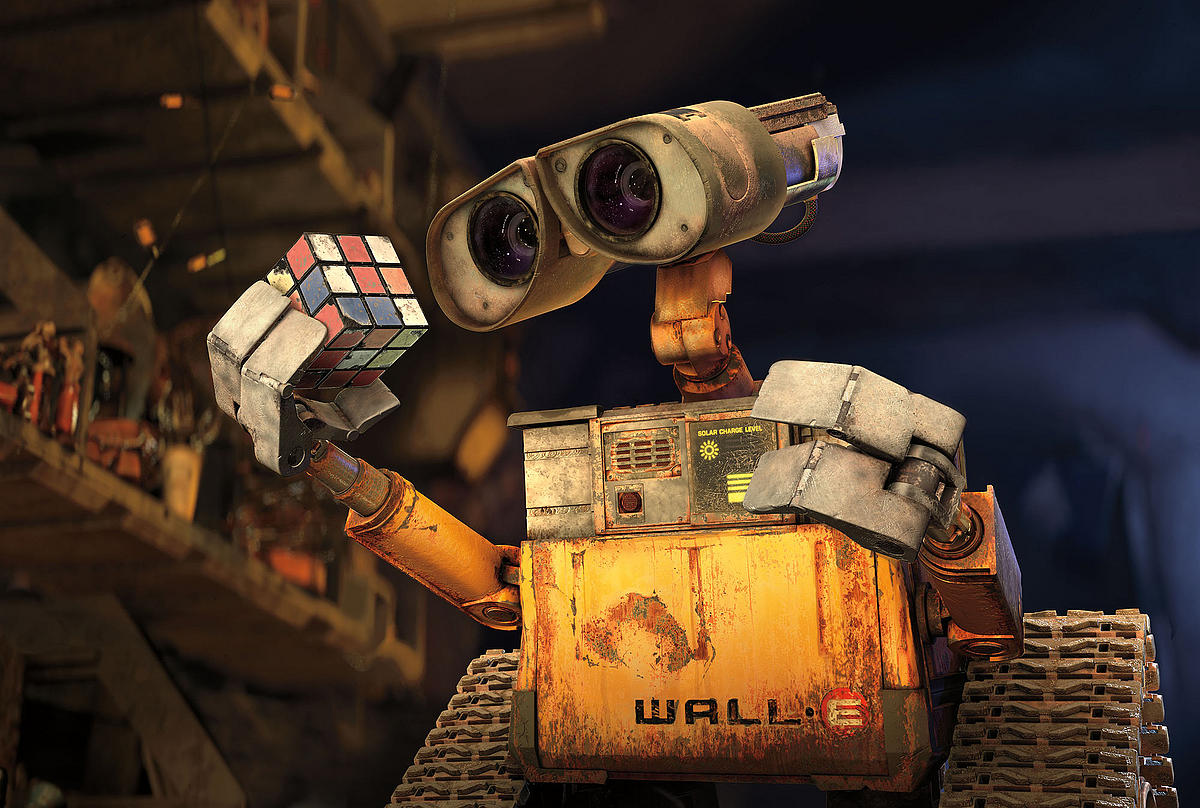
\includegraphics[width=21cm,height=14.8cm]{walle.jpg}};
\end{tikzpicture}
\endpgfgraphicnamed
\end{document}
